\documentclass{article}
\usepackage{blindtext}
\usepackage[a4paper, total={6in, 9.4in}]{geometry}

\usepackage{wrapfig}
\usepackage{graphicx}
\usepackage{mathtext}
\usepackage{amsmath}
\usepackage{siunitx} % Required for alignment
\usepackage{subfigure}
\usepackage{multirow}
\usepackage{rotating}
\usepackage{afterpage}
\usepackage[T1,T2A]{fontenc}
\usepackage[russian]{babel}
\usepackage{caption}
\usepackage[arrowdel]{physics}
\usepackage{booktabs}

\graphicspath{{pictures/}}

\title{\begin{center}Лабораторная работа №3.2.5\end{center}
Вынуденные колебания в электрическом контуре}
\author{Гёлецян А.Г.}
\date{\today}

\begin{document}

\pagenumbering{gobble}
\maketitle
\newpage
\pagenumbering{arabic}

\textbf{Цель работы:} Исследовать вынужденные колебания, возникающие в электрическом
колебательном контуре под воздействием внешней э.д.с., гармонически изменяющейся во
времени.

\section{Теоретическая часть}\label{theory}
\subsection{Резонансная кривая}\label{theory_achx}
\vspace{0.5cm}
\begin{wrapfigure}{l}{0.5\textwidth}
  \begin{center}
    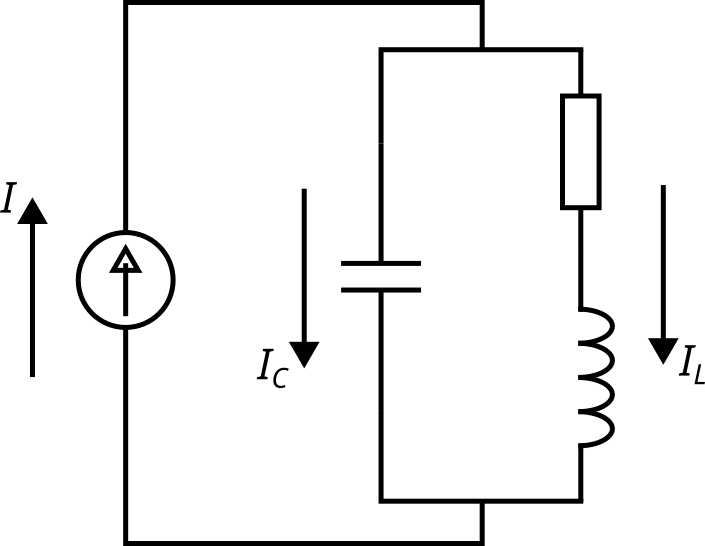
\includegraphics[width=0.48\textwidth]{sxema.png}
  \end{center}
  \caption{Параллельный контур}\label{fig:sxema}
\end{wrapfigure}

Пусть имеется источник тока, который генерирует ток с частотой $\omega$ и комплексной
амплитудой $I$. Тогда, имеем следующие уравнения

\begin{align*}
    I &= I_C + I_l \\
    \frac{I_C}{i\omega C} &= (i\omega L + R) I_L
\end{align*}

Введем обозначения $\rho=\sqrt{L/C}$ и $\omega_0=1/\sqrt{LC}$. Тогда, преобразуя уравнения выше получим

\begin{align*}
    I_C &= \left(-\frac{\omega^2}{\omega^2_0} +i\frac{\omega R}{\omega_0\rho}\right)I_L\\
    I_L &= I\frac{1}{1-\frac{\omega^2}{\omega_0^2} + i \frac{\omega R}{\omega_0 \rho}} = 
        I \frac{-i\frac{\rho\omega_0}{R\omega}}{1+i\frac{\rho}{R}\left(
            \frac{\omega}{\omega_0} - \frac{\omega_0}{\omega}\right)}
\end{align*}
Напряжение на контуре равно $U = (i\omega L + R)I_L$. Приняв обозначение $Q=\rho/R$
распишем выражение для $U$
\begin{equation}
    U = (i\omega L+R)I_L=I\frac{\rho^2}{R}\frac{1 - i\frac{\omega_0/\omega}{Q}}
    {1 + iQ\left(\frac{\omega}{\omega_0} - \frac{\omega_0}{\omega}\right)}
\end{equation}\label{eq:voltage}

При $Q \ge 5$ максимум $\abs{U}$ достигается при $\omega = \omega_0$ с точностью до 
$0.04\%$, поэтому в дальнейшем будем считать, что резонансная частота совпадает с
$\omega_0$. Так же, с хорошей точностью, ширина кривой $\abs{U(\omega)}$ на высоте
$\abs{U(\omega_0)} / \sqrt{2}$ равна $\omega_0/Q$. Благодаря этому факту можно измерить
добротность $Q$ изучая резонансную кривую контура.

\newpage
\subsection{Процессы установления и затухания колебаний в контуре}\label{theory_perexod}
\begin{figure}[h]
    \center{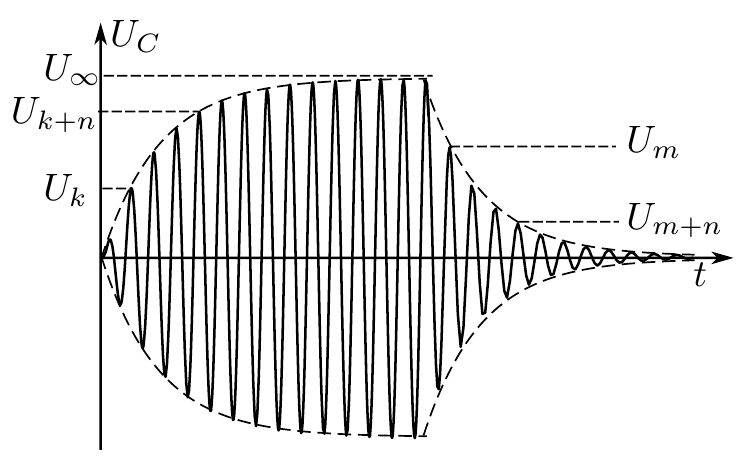
\includegraphics[width=0.7\textwidth]{ustanovlenie_zatuxanie.png}}
    \caption{Нарастание и затухание вынужденных колебаний}\label{fig:ustanovlenie_zatuxanie}
    \newpage
\end{figure}

Общее решение уравнения, описывающей контур, является суммой экспоненциально затухающих
колебании и стабильных вынужденных колебании. Если на разряженный контур начать подавать
внешнее напряжение с резонансной частотой, то амплитуда колебании будет менятся по закону
\begin{equation}
    U(t) = U_{\infty}(1 - e^{-\gamma t})
\end{equation}\label{eq:narastanie}

где $\gamma = R/(2L) = \omega_0 / (2Q)$. Аналогично, если выключить внешнее напряжение,
то останутся только затухающие колебания, и амплитуда будет менятся по закону
\begin{equation}
    U(t) = U_{0}e^{-\gamma t}
\end{equation}\label{eq:zatuxanie}

Таким образом, измеряя зависимость амплитуды от времени можно получить $\gamma$, и, как
следствие, добротность.

\newpage
\section{Ход работы}
\subsection{Измерение резонансной кривой}\label{mes_achx}
\begin{figure}[h]
    \center{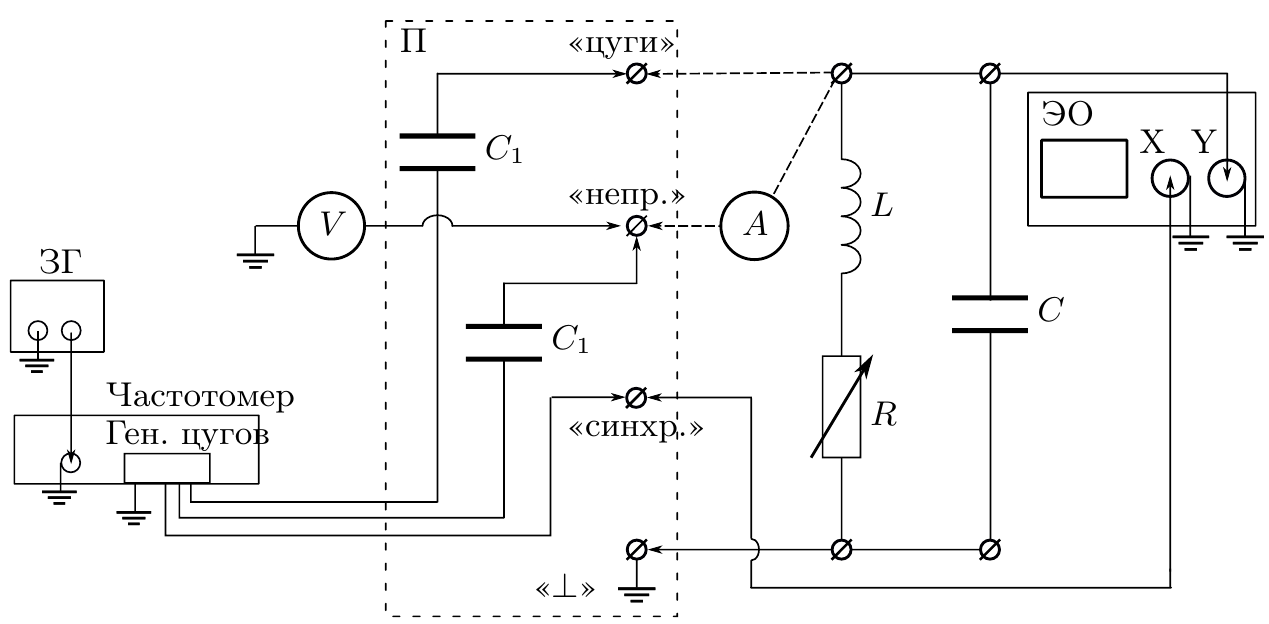
\includegraphics[width=0.7\textwidth]{ustanovka.png}}
    \caption{Установка}\label{fig:ustanovka}
    \newpage
\end{figure}

При изучении резонансной кривой в \ref{theory_achx} мы предполагали, что источник выдает
постоянный ток. Чтобы получить похожее состояние, генератор сигналов подключается к
контуру через маленькую емкость $C_1$, благодаря которому импеданс "нагрузки"
определяется почти полностью импедансом этой емкости $Z_{C_1} = \frac{1}{i\omega C_1}$.

\begin{figure}[h]
    \center{\includegraphics[width=1\textwidth]{achx.eps}}
    \caption{Резонансные кривые для двух значении $R$}\label{fig:achx}
    \newpage
\end{figure}

\newpage
Измерения ширины резонансных кривых на высоте $U/U_0=1/\sqrt{2}$ дают следующие значения
добротностей

\begin{equation}
    \begin{aligned}
        Q_{R=0}^{АЧХ}&=24.8\\
        Q_{R=100\Omega}^{АЧХ}&=6.49
    \end{aligned}
\end{equation}

\subsection{Измерение добротности при помощи процесса установления}\label{mes_perexod}
Во время измерения резонансных кривых мы нашли резонансные частоты контуров. Они
оказались равны в пределах погрешности
$\nu_0^{R=0}=\nu_0^{R=100\Omega}=\nu_0=(1560 \pm 2.5)Гц$. Выставляем на генераторе цугов
эту частоту, и подбираем длительность и период цегов так, чтобы колебания успели
установится и затухнуть соответственно. Результаты измерении можно увидеть на графиках

\begin{figure}[h]
    \center{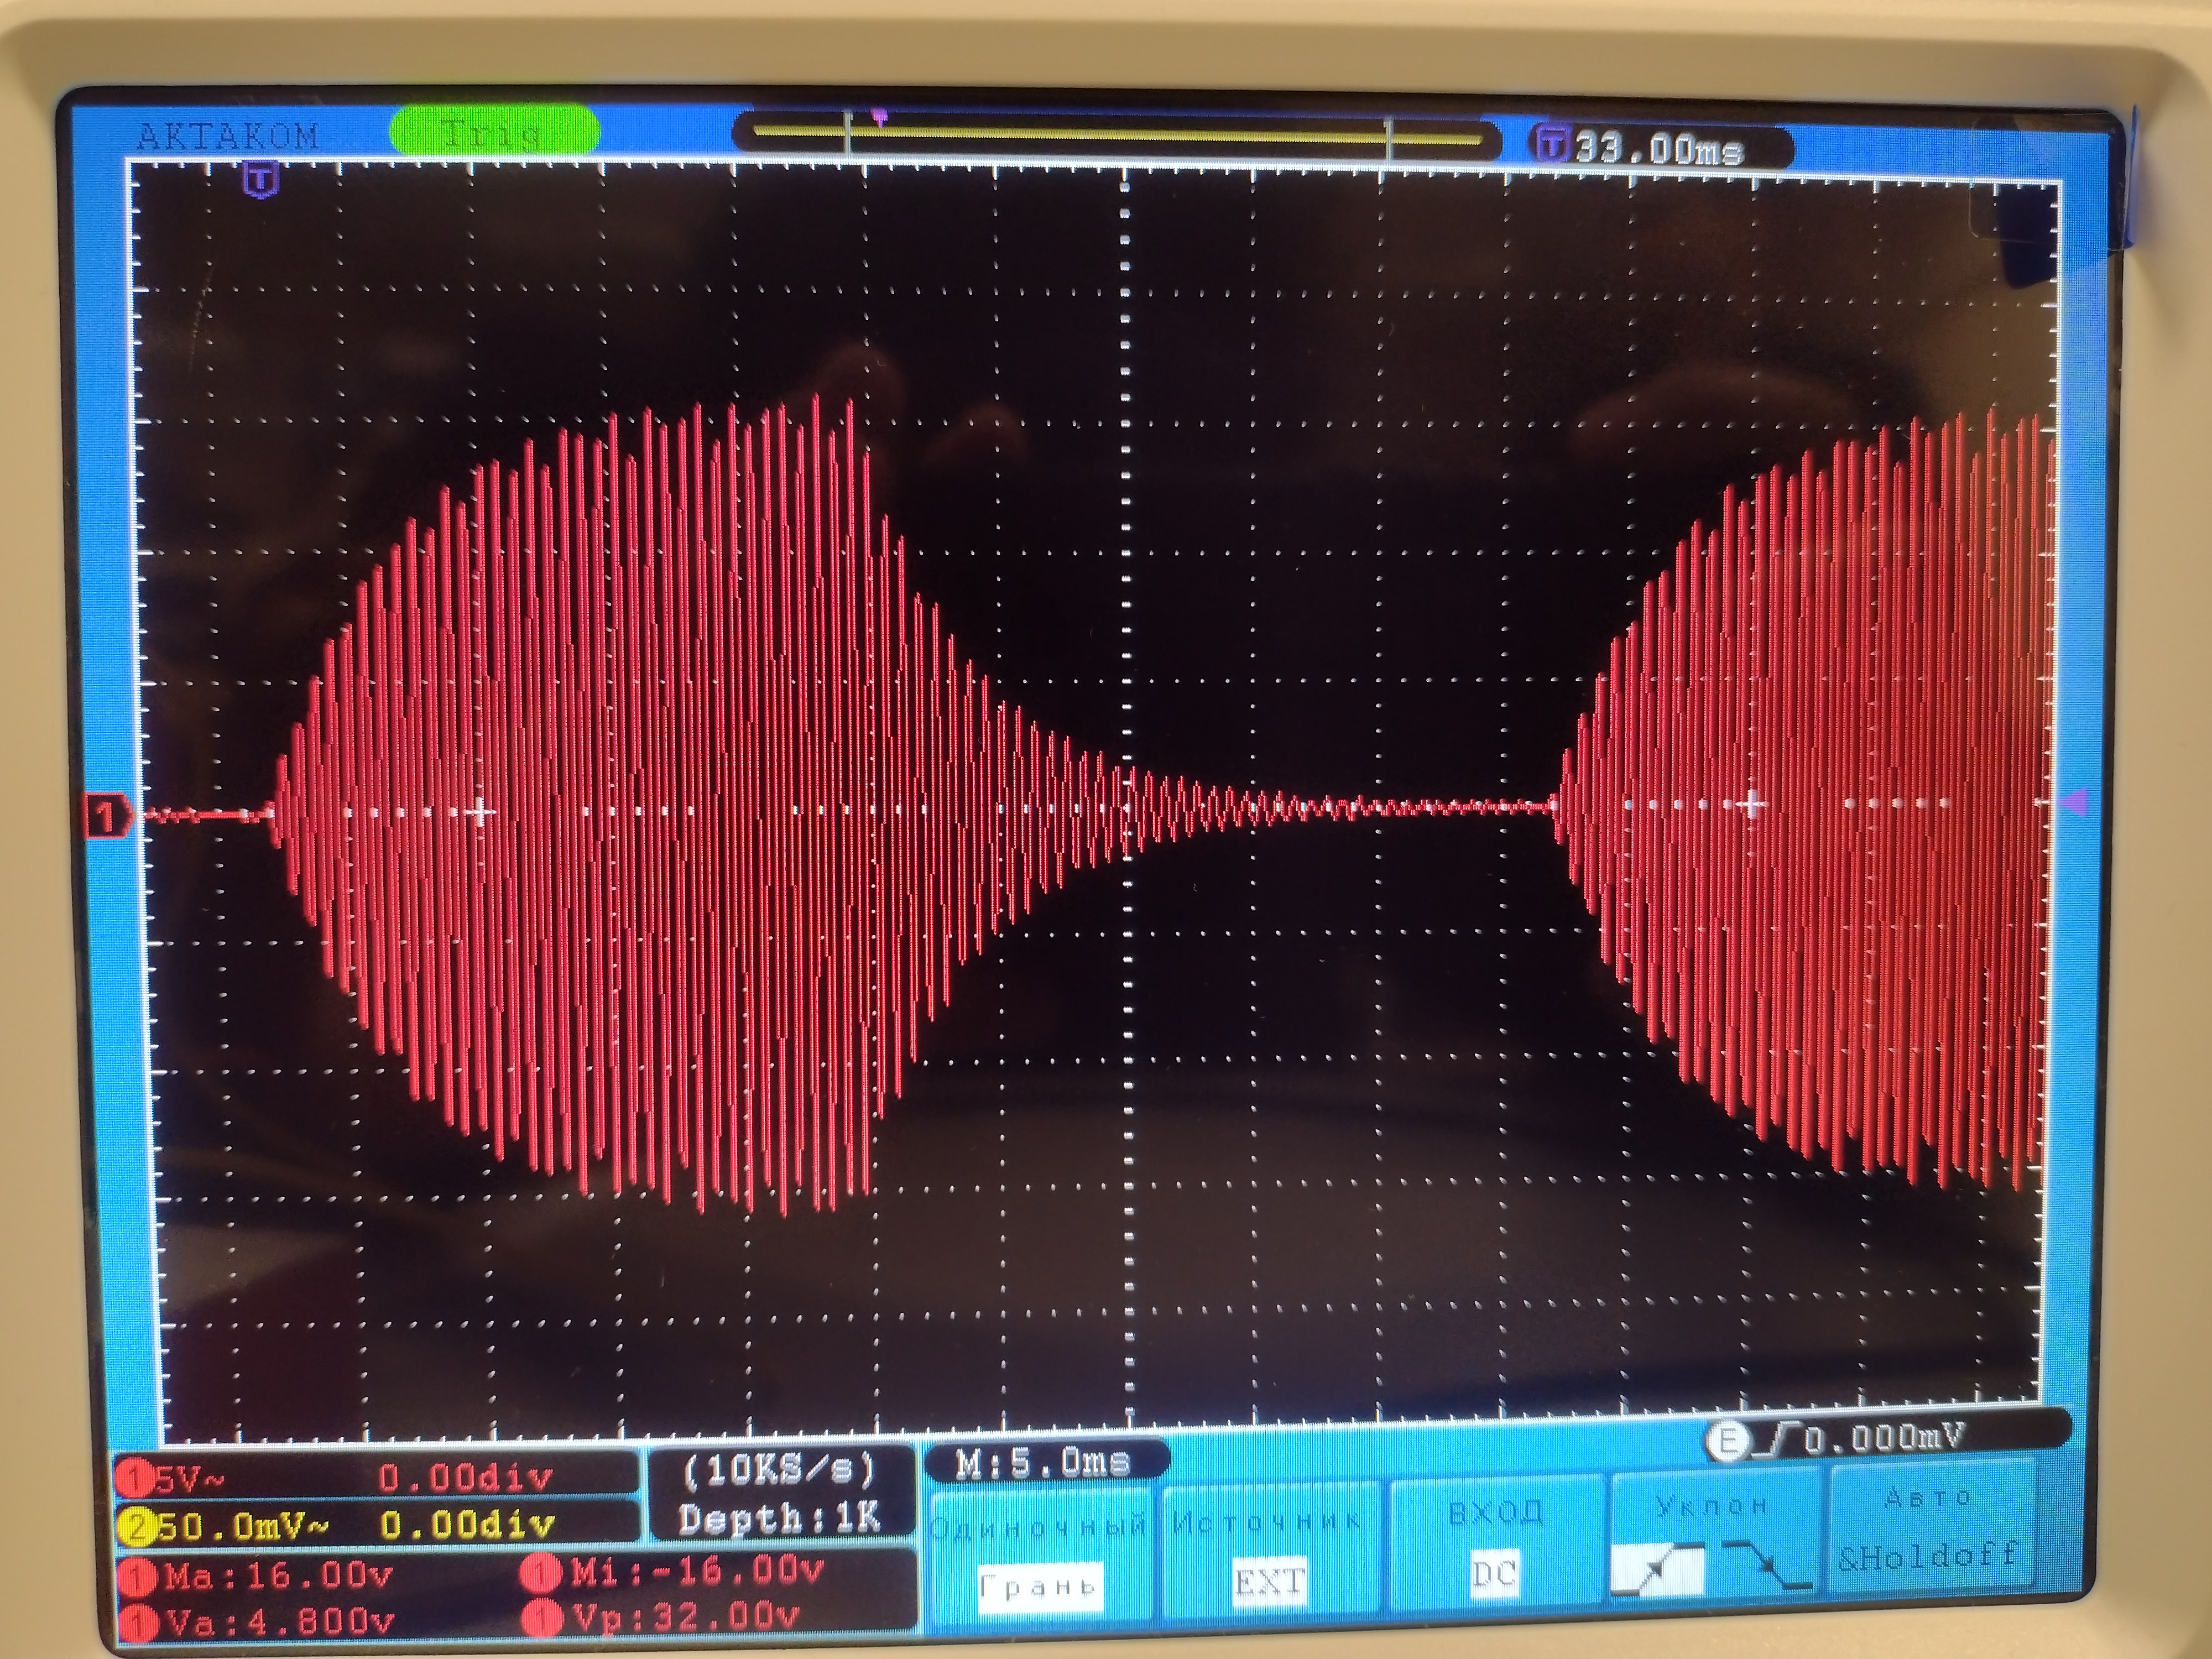
\includegraphics[width=0.4\textwidth]{perexod_oscilloscope.jpg}}
    \caption{Осциллограмма переходного процесса}\label{fig:perexod_oscilloscope}
    \newpage
\end{figure}

\begin{figure}[h]
    \center{\includegraphics[width=1\textwidth]{perexod_R_0.eps}}
    \caption{Переходные процессы для контура с $R=0$}\label{fig:perexod_R_0}
    \newpage
\end{figure}

\newpage

\begin{figure}[h]
    \center{\includegraphics[width=1\textwidth]{R_0_damp.eps}}
    \caption{Линеризованные графики процессов для контура с $R=0$}\label{fig:R_0_damp}
    \newpage
\end{figure}

Из параметров грайика получаем следующие значения

\begin{equation}
    \begin{aligned}
        Q_{R=0}^{уст} &= 23.8 \pm 0.5 \\
        Q_{R=0}^{затух} &= 23.70 \pm 0.16
    \end{aligned}
\end{equation}

\vspace{1cm}

Повторим эксперимент для контура с $R=100\Omega$. Получаем значения

\begin{equation}
    \begin{aligned}
        Q_{R=100\Omega}^{уст} &= 6.8 \pm 0.7 \\
        Q_{R=100\Omega}^{затух} &= 6.79 \pm 0.09
    \end{aligned}
\end{equation}



\newpage

\begin{figure}[h]
    \center{\includegraphics[width=0.81\textwidth]{perexod_R_100.eps}}
    \caption{Переходные процессы для контура с $R=100\Omega$}\label{fig:perexod_R_100}
    \newpage
\end{figure}

\begin{figure}[h]
    \center{\includegraphics[width=0.81\textwidth]{R_100_damp.eps}}
    \caption{Линеризованные графики процессов для контура с $R=100\Omega$}\label{fig:R_100_damp}
    \newpage
\end{figure}

\newpage

Если на вход контура подать цуги частоты, близкой к резонансной, то получится сумма
двух синусов с близкими частотами, один из которых затухает во времени. В результате
увидим биения, скважность которых уменьшается со временем.

\begin{figure}[h]
    \center{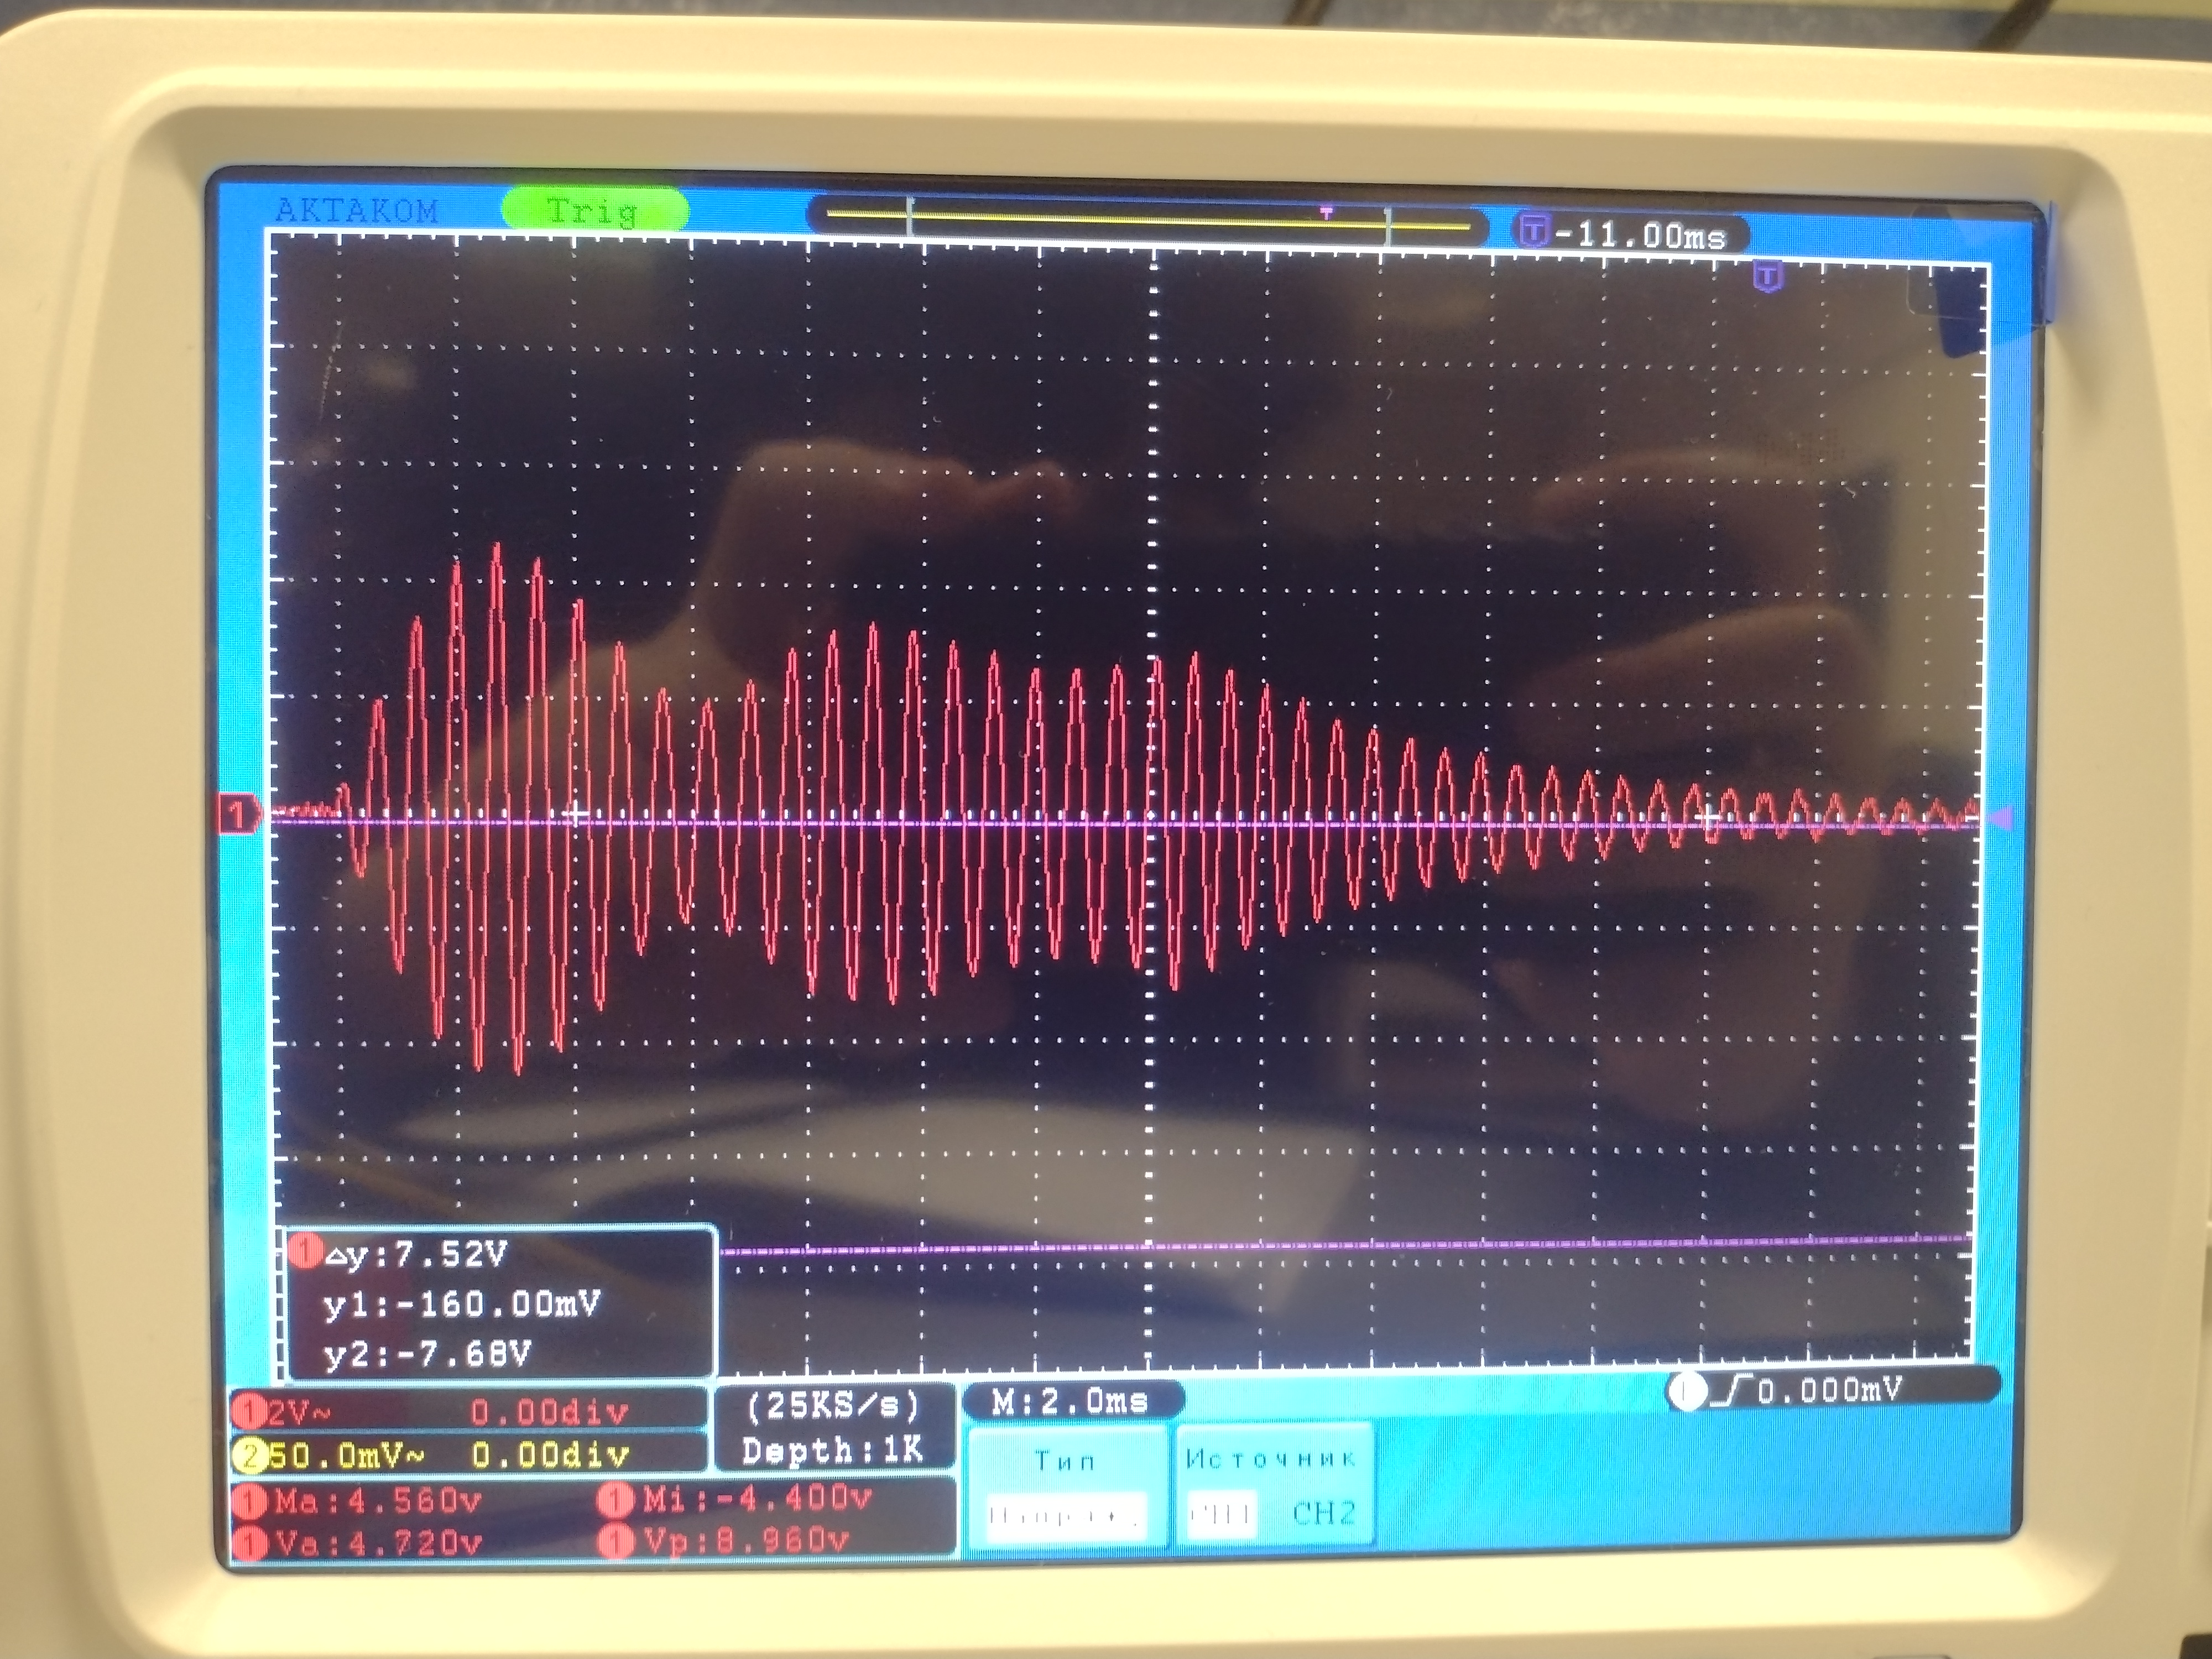
\includegraphics[width=\textwidth]{bieniya.jpg}}
    \caption{Биения при $\nu=1400 Гц$, $R=0$}\label{fig:bieniya}
    \newpage
\end{figure}

\subsection{Подведение результатов}\label{results}
При помощи RLC-метра измерим индуктивность и сопротивление индуктивности
\begin{align*}
    L_{\nu=5кГц} =&\ 99.631 мГн &L_{\nu=1.5кГц} =& \ 98.978 мГн\\
    R_{\nu=5кГц} =&\ 42.7 \Omega & R_{\nu=1.5кГц} =&\  29.7 \Omega\\
\end{align*}

Как видим, индутивность слабо зависит от частоты, но сопротивление меняется значительно
из за скин-эффекта. Наши измерения проводились около резонансной частоты $\nu_0=1560Гц$,
поэтому сопротивление катушки будем брать $R_L=29.7\Omega$, $L=98.978мГн$,
$C=0.1\mu Ф \pm 3\%$. Получаем следующие результаты

\begin{table}[!h]
\begin{center}
\begin{tabular}{llllll}
$R, \Omega$ & $R_{контур}, \Omega$ & $Q^{АЧХ}$ & $Q^{уст}$ & $Q^{затух}$ & $Q^{теор}$ \\
\toprule
0   &  29.7  & 24.8  & 23.8 $\pm$ 0.5  & 23.70 $\pm$ 0.16 & 33.5   \\
100 & 129.7  & 6.49  & 6.8  $\pm$ 0.7  & 6.79  $\pm$ 0.09 & 7.67      
\end{tabular}
\end{center}
\end{table}

\newpage
\section{Выводы}\label{vivodi}
Судя по результатам, самый точный метод измерения добротности это измерение по скорости
затухания. Как видим теоретические значения не совпадают с реальностью. Это может
быть обусловлена неточностью измерения сопротивления контура - скин-эффект, сопротивления
проводов, сопротивление конденсатора. Факторов много, учесть все не получиться, но можно
проверить гипотезу, зная что разница сопротивлений в контурах $100\Omega$. Из уравнения
для $Q$ имеем

\begin{equation}
    R = \frac{1}{Q} \sqrt{\frac{L}{C}}
\end{equation}

Подставляем наши значения, взяв за $Q$ значения, измеренные при помощи скорости затухания

\begin{equation}
    \begin{aligned}
        R_{контур}^{R=0} &= (42.0 \pm 0.7) \Omega \\
        R_{контур}^{R=100\Omega} &= (146 \pm 3) \Omega \\
    \end{aligned}
\end{equation}

Как видим, эти значения отличаются на $102\Omega$, что достаточно близко к ожидаемому
значению. Отсюда делаем вывод, что несоответствия с теорией нет, просто мы не смогли
измерить сопротивление контура так как надо.
\end{document}

